\section{Sintonía PID en Lazo Abierto (Ziegler--Nichols, método de respuesta al escalón)}

El método consiste en analizar la respuesta al escalón de la planta en lazo abierto, identificar el punto de \emph{máxima pendiente} y trazar la tangente en ese punto. A partir de las intersecciones de esa recta con el nivel inicial (0) y el valor final \(K=\mathrm{dcgain}(G)\), se obtienen los parámetros \(\,L\,\) (tiempo muerto aparente) y \(\,T\,\) (constante aparente) del modelo. Con \(L\) y \(T\) se definen las ganancias iniciales del PID según Ziegler--Nichols.

Para esto se utilizó el siguiente script de MatLab:
\onecolumn
\subsection{Script utilizado}
\begin{lstlisting}[language=Matlab,style = matlabstyle, caption={ZN por respuesta al escalon: extraccion de L y T y calculo de PID}, label={lst:zn_step}, frame=single]
	% ======= Step Response Method (ZN) =======
	[L, T, S, t_max] = zn_step_params(G, ts, wn);
	K = 1; % dcgain(G);  % en este caso es 1
	
	K_zn_step  = 1.2*T/(K*L);
	Ti_zn_step = 2*L;
	Td_zn_step = 0.5*L;
	
	numC = K_zn_step*[Ti_zn_step*Td_zn_step, Ti_zn_step, 1];
	denC = [Ti_zn_step, 0];
	C = tf(numC, denC);
	
	cl_zn_step = feedback(C*G, 1);
	step(cl_zn_step)
	fprintf("Inicial ZN-step: Kp=%.3g Ti=%.3g Td=%.3g\n",K_zn_step,Ti_zn_step,Td_zn_step);
	
	function [L, T, S, t_max] = zn_step_params(G, ts, wn)
	% ZN_STEP_PARAMS  Ziegler-Nichols (step response)
	t_end = 1.1*ts;
	if ~isfinite(t_end) || t_end<=0, t_end = 5*(1/wn); end
	N = max(1000, round(5000*(2*pi/wn)));
	t = linspace(0, t_end, N);
	[y, tout] = step(G, t);
	K = dcgain(G); if ~isfinite(K), K = y(end); end
	dy = gradient(y, tout);
	[S, idx] = max(dy); idx = idx(1);
	t_max = tout(idx); y_max = y(idx);
	% Tangente: y_tan = y_max + S*(t - t_max)
	L = t_max - y_max/S;       % corte con y=0
	T = K / S;                 % tiempo adicional hasta K
	% (Graficas opcionales)
	end
\end{lstlisting}

\twocolumn

La función genera como salida la respuesta al escalón de la planta junto con la tangente en el punto de máxima pendiente, señalando los valores de \(L\) y \(L+T\). En la Figura~\ref{fig:zn_step_out} se muestra la gráfica exportada desde Matlab.

\begin{figure}[!t]
	\centering
	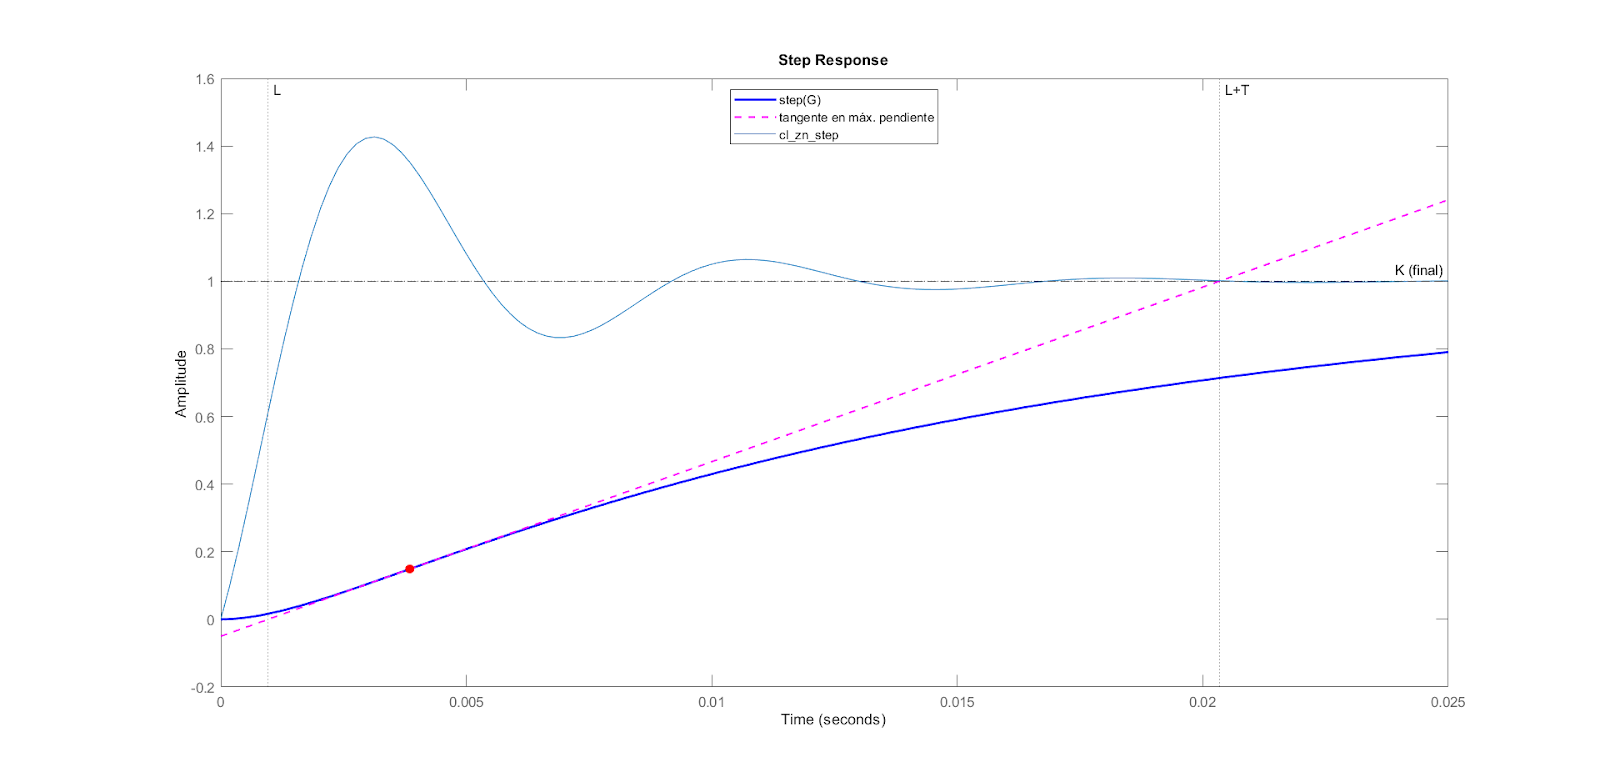
\includegraphics[width=\columnwidth]{img/zn_step_response.png} % <-- coloca aquí tu imagen exportada
	\caption{Respuesta al escalón en lazo abierto con la tangente en el punto de máxima pendiente y la Respuesta al escalon en lazo cerrado usando los valores de \(K_p,T_i\) y \(T_d\) obtenidos por el metodo.}
	\label{fig:zn_step_out}
\end{figure}

\subsubsection*{Cálculo de \(K\), \(L\) y \(T\)}
\begin{itemize}
	\item La ganancia estática del sistema \(K\) se obtiene como el valor final de la salida ante un escalón unitario, es decir \(K = \mathrm{dcgain}(G)\). En nuestro caso, \(K=1\).
	\item El tiempo muerto aparente \(L\) corresponde a la intersección de la tangente (en el punto de máxima pendiente) con el eje tiempo cuando la salida es cero.
	\item La constante aparente \(T\) se obtiene como el tiempo adicional que tarda esa misma tangente en alcanzar el valor final \(K\). Equivalentemente, \(T = K/S\), siendo \(S\) la pendiente máxima.
\end{itemize}

\begin{table}[!t]
	\centering
	\small
	\caption{Reglas de Ziegler--Nichols por respuesta al escalón.}
	\label{tab:zn_rules}
	\resizebox{0.7\columnwidth}{!}{%
		\begin{tabular}{l c c c}
			\toprule
			\textbf{Controlador} & $K_p$ & $T_i$ & $T_d$ \\
			\midrule
		P   & $T/(K\,L)$      & --   & -- \\
		PI  & $0.9\,T/(K\,L)$ & $3L$ & -- \\
		PID & $1.2\,T/(K\,L)$ & $2L$ & $0.5L$ \\
		
			\bottomrule
		\end{tabular}%
	}
\end{table}


Aplicando este método a nuestra planta se encontró:
\[
L = 9.64 \times 10^{-4}~\text{s}, \quad T = 1.94\times 10^{-2}~\text{s}, \quad K=1.
\]
Y utilizando la tabla \ref{tab:zn_rules} podemos obtener los siguientes valores iniciales:
\[
K_p = 24.1, \qquad T_i = 0.00193~\text{s}, \qquad T_d = 0.000482~\text{s}.
\]

En la Figura~\ref{fig:zn_step_out} se muestra la respuesta obtenida con los valores de $K_p$, $T_i$ y $T_d$ calculados. 
Por su parte, en la Tabla~\ref{tab:resultadosPID} se resumen las principales métricas de desempeño del sistema: \emph{overshoot}, tiempo de subida y tiempo de establecimiento.

